\documentclass{article}
\usepackage{graphicx}
\usepackage{geometry}
\usepackage{hyperref}
\usepackage{xcolor}
%%\usepackage{showframe}
\geometry{left=80pt,right=80pt,top=40pt,bottom=40pt}

\renewcommand*\contentsname{Table Des Matières}

\begin{document}
	\author{Thivagini SUGUMAR, Marine CONOR}
	\date{3 décembre 2023}
	
	\title{\underline{\textbf{M2 DataScale}}\\
		\bigskip
		\textbf{TP - Architectures Orientées Service}\\
		\bigskip
		Spécification du Service Web Composite : Evaluation de Demande de Prêt Immobilier
		\bigskip}
	
	\maketitle
	\newpage
	\tableofcontents
	\newpage
	
	\section{Contexte général du TP}
	Le service Web Composite d'Évaluation de Demande de Prêt Immobilier est conçu pour automatiser le processus d'évaluation des demandes de prêt immobilier en utilisant des services Web spécialisés. 
	\newline Il permet aux clients de soumettre des demandes de prêt immobilier exprimées en langage naturel. Le service intègre des composants d’extraction des informations métiers de texte de la demande, de vérification de solvabilité, d'évaluation de la propriété et de décision d'approbation pour fournir une évaluation complète et précise des demandes de prêt. 
	
	\section{Objectif}
	L'objectif de ce service est de fournir une interface unique pour les clients qui souhaitent demander un prêt immobilier. Le service coordonne les différents services Web nécessaires pour évaluer la demande du client, garantissant ainsi un processus fluide et automatisé.
	
	
	\section{Fonctionnement du système}
	\subsection{Architecture}
	Nous représentons l’architecture du fonctionnement du système par le diagramme suivant : 
	\\
	\\
		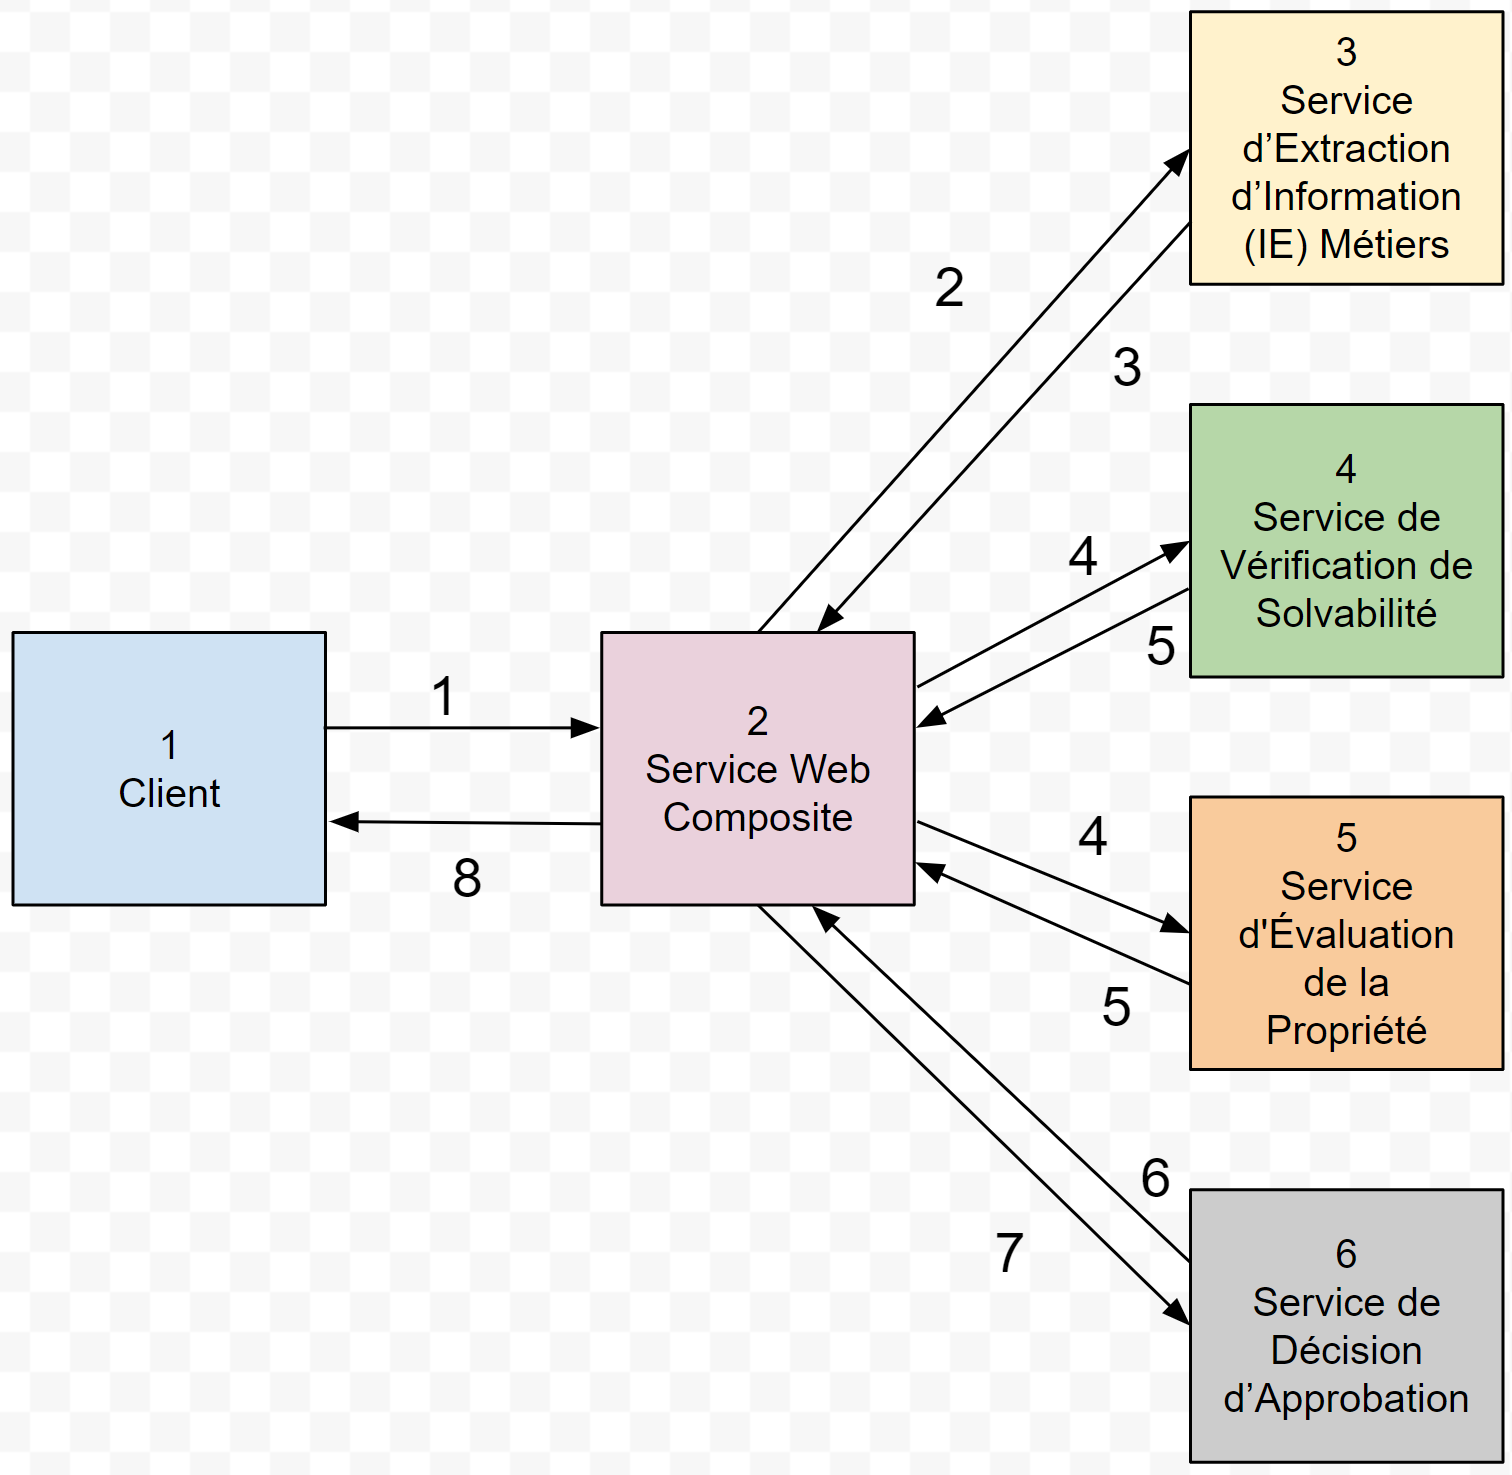
\includegraphics[width=\textwidth]{images/architecture.png}
	\subsection{Étapes}
	  \begin{itemize}
	  	\item Sur l’interface, le client va effectuer une demande de prêt. Pour cela, le client doit remplir un formulaire et le soumettre. Cette action va permettre de créer un fichier sous format \texttt{txt} dans le répertoire \texttt{demandeTxt}
	  	
	  	\item Le service \textbf{Composite} va détecter l’arrivée du fichier \texttt{txt} dans le répertoire \texttt{demandeTxt} grâce à une routine qui se lance automatiquement. Ainsi le service composite va récupérer ce fichier \texttt{txt}
	  	
	  	\item Le service composite va effectuer une requête au service \textbf{Extraction} afin de récupérer le fichier WSDL
	  	
	  	\item Le service composite va alors transmettre le fichier \texttt{txt} au service d’\textbf{Extraction} via sa méthode web service encapsulé dans une enveloppe SOAP
	  	
	  	\item Le service d’\textbf{Extraction} va effectuer le prétraitement, identifier des entités et extraire les entités avec les expressions régulières. Cette extraction sera sauvegardée dans un fichier \texttt{XML} dans \texttt{demandeXML} sous le format : \texttt{numeroDossier.xml}
	  	
	  	\item Le service d’\textbf{Extraction} renvoie ce fichier \texttt{XML} obtenu au service \textbf{Composite}
	  	
	  	\item Le service \textbf{Composite} donne le fichier \texttt{XML} au service de \textbf{Vérification de Solvabilité}
	  	
	  	\item Le service de \textbf{Vérification de Solvabilité} va utiliser une fonction de scoring pour donner un score. Il ajoute les balises \texttt{<scoring></scoring>} et \texttt{<decisionScoring></decisionScoring>} dans le fichier \texttt{XML}
	  	
	  	\item Le service de \textbf{Vérification de Solvabilité} renvoie le fichier \texttt{XML} modifié au service \textbf{Composite}
	  
	  	\item Le service \textbf{Composite} donne le fichier \texttt{XML} modifié au service d'\textbf{Évaluation de la Propriété}
	  	
	  	\item Le service d'\textbf{Évaluation de la Propriété} va utiliser une fonction pour évaluer le marché immobilier afin de donner une moyenne et évaluer les normes légales et réglementaires du bâtiment. \\
	  	Il peut aussi décider de faire une visite virtuelle et une visite sur place. \\
	  	Il ajoute les balises : \\
	  	\texttt{<estimation\_valeur></estimation\_valeur>} et \\
	  	 \texttt{<decisionConformite></decisionConformite>}, si la décision est "Non admissible". \\
	  	Il ajoute également aussi une balise \texttt{<raisons></raisons>} dans le fichier \texttt{XML} donné en entrée
	  	
	  	\item Le service d'\textbf{Évaluation de la Propriété} renvoie le fichier \texttt{XML} modifié au service \textbf{Composite}
	  	
	  	\item Le service \textbf{Composite} donne le fichier \texttt{XML} modifié au service de \textbf{Décision d'Approbation}
	  	
	  	\item Le service de \textbf{Décision d’Approbation} va utiliser une fonction comparant les résultats et analyses précédents. Il va ensuite créer un nouveau fichier \texttt{txt} dans le dossier \texttt{reponseTxt} sous le format \texttt{numeroDossier.txt}
	  	
	  	\item Le service de \textbf{Décision d’Approbation} renvoie le fichier \texttt{txt} au service \textbf{Composite}
	  	
	  	\item Le client peut retrouver sa réponse sur l’interface en consultant les résultats
	  	
	  \end{itemize}
	
	\newpage
	\section{Identification des services}
		Les services identifiés sont les suivants : \\
		
		\begin{itemize}
			\item Le service \textbf{Composite} : \\
			
			Permet l’interaction entre le Client et les différents Services. Il s’occupe notamment de la réception de la demande, l’extraction d’information métier, la vérification de solvabilité, l’évaluation de la propriété et la décision d'approbation.
			
			\item Le service d’\textbf{Extraction} : \\
			
			Reçoit le texte de la demande de prêt soumise par le client, via le service \textbf{Composite}. \\
			Il s’occupe principalement du prétraitement, analyse, identification des entités et l’extraction de ces informations. De plus, il permet le stockage des informations extraites dans la base de données du service \textbf{Composite}
			
			\item Le service de \textbf{Vérification de Solvabilité} : \\
			
			Permet d'évaluer la capacité financière du client à rembourser le prêt. Il s’occupe donc de l’intégration des bureaux de crédit pour se connecter à leurs bureaux qui stockent l'historique financier des clients. Il récupère des informations telles que les dettes en cours, les paiements en retard et les antécédents de faillite pour évaluer la crédibilité du client. Ensuite, le service utilise des algorithmes de scoring de crédit pour attribuer un score au client en fonction de son historique financier. Ce score représente le niveau de risque associé à l'accord d'un prêt au client. Les clients avec des scores élevés ont une solvabilité plus élevée. Il analyse aussi les revenus et les dépenses mensuelles.
			
			\item Le service d'\textbf{Évaluation de la Propriété} :\\
			
			Permet d'estimer la valeur marchande de la propriété pour laquelle le prêt est demandé. Il peut utiliser des données immobilières, des expertises locales et des critères légaux pour effectuer cette évaluation. Il s’occupe donc d'analyser les données du marché immobilier, peut effectuer une inspection virtuelle de la propriété ou même des visites sur place et vérifier si la propriété est conforme aux normes légales et réglementaires en vigueur.
			
			\item Le service de \textbf{Décision d'Approbation} : \\
			
			Analyse les données recueillies lors des étapes précédentes (Vérification de Solvabilité et Évaluation de la Propriété) pour déterminer si le prêt immobilier peut être approuvé. Il s’occupe d’analyser les risques associés à l'accord du prêt, de comparer les données de la demande de prêt avec les politiques internes de l'institution financière pour évaluer la probabilité de défaut de paiement du client. En fonction des résultats, le service prend une décision d'approbation ou de refus du prêt puis communique celle-ci au service \textbf{Composite} (en indiquant les raisons de l'approbation ou du refus du prêt) qui va retourner cette réponse au client.
			
		\end{itemize}
	
	\newpage
	\section{Modélisation des services}
	\subsection{Modélisation}
	Une architecture à base de service pour mettre en œuvre le processus d’évaluation de demande de prêt immobilier :
	\\
	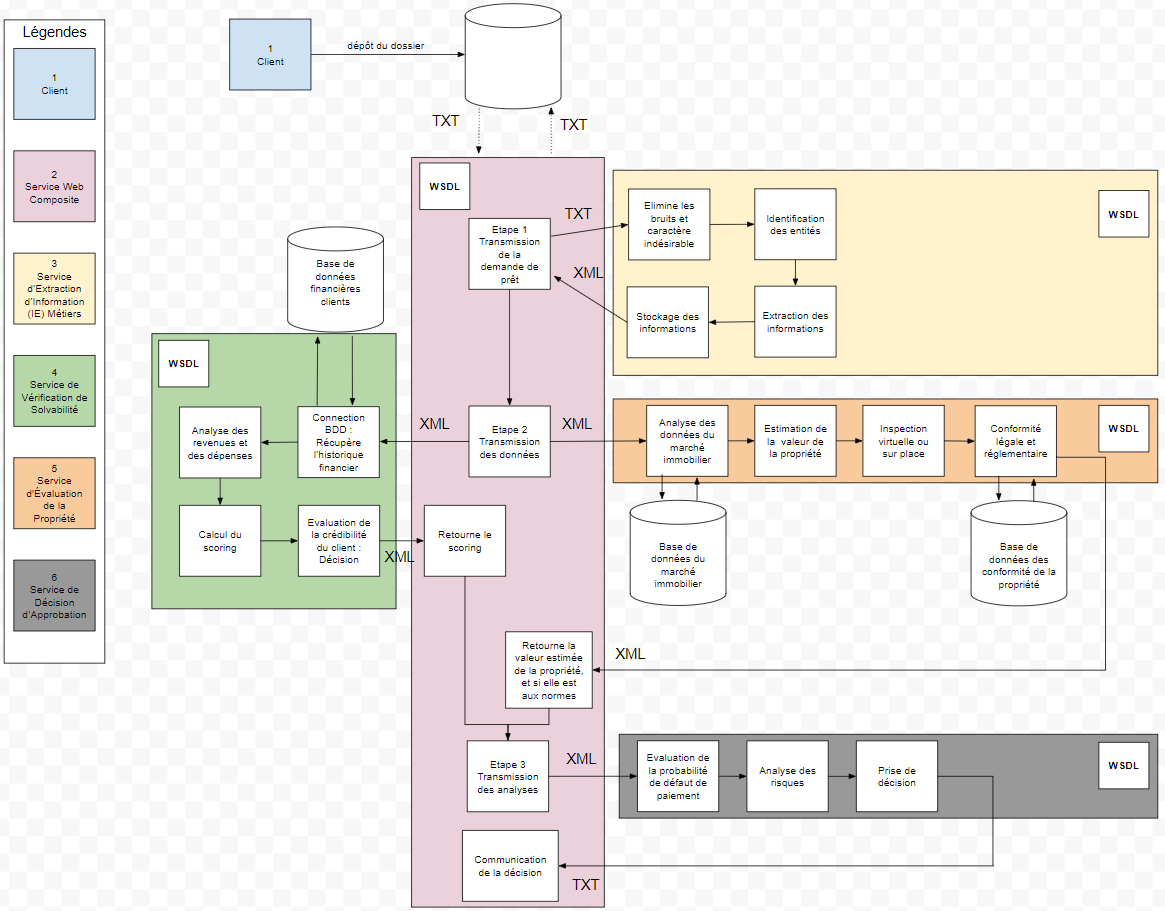
\includegraphics[width=\textwidth]{images/modelisation_XML.png}
	
	\newpage
	\subsection{Fonctionnement interne des services}
	Le service \textbf{Composite} permet les échanges entre les services et les échanges avec le client et organise le SOAP. \\
	\\
	Le service d’\textbf{Extraction} prend en paramètre le fichier \texttt{txt} de la demande du client.\\
	Ce service va récupérer les informations indiquées dans le fichier \texttt{txt}, supprime les caractères indésirables et extrait les données après le caractère " : ".\\
	Une fois extraites, les données sont écrites dans des balises correspondantes dans un fichier \texttt{XML}. \\
	Le fichier XML sera nommé selon le numéro de dossier attribué au client. \\
	\\
	Le service de \textbf{Vérification de Solvabilité} prend en paramètre le fichier \texttt{XML} concernant la demande du client. \\
	Ce service va récupérer les informations concernant le montant et la durée du prêt ainsi que les revenus et les dépenses mensuelles à l'aide du numéro de dossier du client. \\
	Il va également récupérer le fichier \texttt{json} banque : \\
	(\texttt{idBanque, age, enfants, emploi, nbCreditsEnCours, antecedents, tauxEndettement}) où : 
	\begin{itemize}
		\item \texttt{idBanque} est l’identifiant de la banque du client
		\item \texttt{age} est l’âge du client
		\item \texttt{enfants} est le nombre d’enfants à sa charge
		\item \texttt{emploi} est un booléen avec 0 si l’emploi n’est pas stable, 1 sinon
		\item \texttt{nbCreditsEnCours} est le nombre de crédits totaux toujours en cours
		\item \texttt{antecedents} est le nombre d’antécédents à son actif (dettes non payées, retards…) 
		\item \texttt{tauxEndettement} est le taux d’endettement actuel
	\end{itemize}
	Le service va ensuite extraire les données en prenant le tuple correspondant à l’\texttt{idBanque} du fichier \texttt{XML} et faire un scoring en fonction des informations. \\
	La décision sera immédiatement "Non Admissible" si le client a moins de 18 ans ou si sa capacité d’emprunt ajouté à ses dépenses est supérieure à son revenu ou encore si son taux d’endettement est supérieur à 33\%.\\
	Une fois l’algorithme de scoring effectué, le service va déterminer en fonction du score, une décision : 
	\begin{itemize}
		\item entre 0 et 10 : peu probable
		\item entre 10 et 20 : à défendre
		\item entre 20 et 30 : sous conditions
		\item  entre 30 et 40 : très favorable
	\end{itemize}
	Finalement, le service ajoute au fichier \texttt{XML} reçu, les balises \texttt{<scoring>Valeur du score</scoring>} et \texttt{<decisionScoring>Decision en fonction du score</decisionScoring>}.\\
	
	\newpage
	
	Le service  d'\textbf{Évaluation de la Propriété} prend en paramètre le fichier \texttt{XML} selon la demande du client. \\
	Le service vérifie si la propriété est conforme aux normes légales et réglementaires en vigueur. \\
	Il va pour cela, récupérer l’adresse de la propriété puis récupérer le fichier \texttt{json} immobilier : \\
	(\texttt{idImmobilier, adresse, age, normeLegal, normeReglementaire, litigesEnCours,\\ normeElectricite, normeGaz}) où : 
	\begin{itemize}
		\item \texttt{idImmobilier} est l’identifiant de la propriété
		\item \texttt{adresse} est l’adresse de la propriété
		\item \texttt{age} est l’âge de la propriété
		\item \texttt{normeLegal} est un booléen avec 0 si la propriété est aux normes, 1 sinon
		\item \texttt{normeReglementaire} est un booléen avec 0 si la propriété est aux normes, 1 sinon 
		\item \texttt{litigesEnCours} est le nombre de litiges en cours
		\item \texttt{normeElectricite} est la norme électrique ("NFC 15-100", "NF C 15-100" ou "C 15-100")
		\item \texttt{normeGaz} est la norme pour le gaz (‘NF P 45-500’ ou vide s’il n’y a pas de gaz dans la propriété)
	\end{itemize} 
	
	Le service va ensuite extraire les données en prenant le tuple correspondant à l’adresse du fichier \texttt{XML} et vérifier que tout est conforme : soit 0, soit dans les normes définies. \\
	Si l’un des attributs n’est pas aux normes, la décision est "Non Admissible à un prêt" et liste les raisons pour lesquelles la propriété pose problème. \\
	Il ajoute au fichier \texttt{XML} reçu la balise : \\
	\\
	\texttt{<decisionConformite>\\
	Decision en fonction du respect ou non des normes\\
	</decisionConformite>} \\
	\\
	Si la décision est "Non admissible", il ajoute aussi une balise : \\
	\\
	\texttt{<raisons>Liste des raisons du refus</raisons>}.\\
	\\
	Le service peut demander à faire une visite virtuelle ou sur place, on considère que si le service demande une visite, il effectue d'abord une visite virtuelle, si celle-ci n’est pas concluante, il demande alors un expert pour une visite sur place. \\
	Le service va choisir un entier aléatoire entre 0 et 1 pour savoir s’il fait une visite. \\
	Si  c’est 0, il ne fait aucune demande de visite, sinon il enclenche une visite virtuelle. \\
	Par la suite, on suppose qu’il va faire une visite sur place uniquement si l'âge de la propriété est inférieur à 10 ans (il n’est plus nécessaire d’avoir un certificat de conformité si la propriété a plus de 10 ans). \\
	En fonction des résultats précédents vis-à-vis de la conformité, la visite sur place est déterminée concluante ou non.\\
	Le service va aussi estimer la valeur marchande de la propriété pour laquelle le prêt est demandé. \\
	Il va récupérer le code postal de l’adresse puis récupérer le type de bâtiment (maison/appartement) et, s'il est donné, le nombre d’étages, avec la \texttt{descriptionPropriete} du fichier \texttt{XML}. \\
	Ensuite il récupère le fichier \texttt{json} \texttt{marcheImmobilier} : \\ 
	(\texttt{adresse, codePostal, batiment, nbEtage, valeur}) où : 
	\begin{itemize}
		\item \texttt{adresse} est l’adresse de la propriété
		\item \texttt{codePostal} est le code postal
		\item \texttt{batiment} est le type de bâtiment
		\item \texttt{nbEtage} est le nombre d’étages
		\item \texttt{valeur} est la valeur marchande de la propriété
	\end{itemize}
	Le service va récupérer tous les tuples qui correspondent au même code postal que celui du fichier \texttt{XML} ainsi que le même type de bâtiment, le nombre d’étages s’il est donné et faire une moyenne de leur valeur. \\
	Finalement, il ajoute au fichier \texttt{XML} reçu, la balise :\\
	\texttt{<estimation\_valeur> \\
	Valeur moyenne des bâtiments du même type et dans le même secteur\\
	</estimation\_valeur>}\\
	\\
	Le service  de \textbf{Décision d’Approbation} prend en paramètre le fichier \texttt{XML} concernant la demande du client. \\
	Ce service va récupérer les informations concernant le montant du prêt, le score, la décision du score, la décision de conformité (les raisons pour lesquelles c’est un refus si c'en est un) ainsi que l’estimation de la valeur. 
	\begin{itemize}
		\item Si la valeur du score est -1, le score n’a pas été calculé à cause de sa situation financière, le prêt est refusé.
		\item Si la décision de conformité est "Non admissible à un prêt immobilier", le service émet le refus du prêt avec une liste de raisons.
		\item Si le montant est supérieur à l’estimation de la valeur en plus d'une valeur choisie arbitrairement, le service émet un refus avec les raisons que le montant demandé est trop important pour la propriété.
	\end{itemize}
	
	Par la suite en fonction de la décision du score, \\
	s’il s’agit de "Très favorable", "Sous conditions" ou "À défendre" et que la décision de conformité est aussi "Admissible à un prêt immobilier" alors le service accepte la demande, sinon il la refuse.\\
	En fonction des résultats précédents, le service a pris une décision d'approbation ou de refus du prêt puis communique celle-ci au service \textbf{Composite} (en indiquant les raisons du refus du prêt) sous la forme d’un fichier \texttt{txt} qui sera stocké dans le répertoire \texttt{reponseTxt}.
	
	\newpage
	\section{Implémentation avec SOAP}
	\subsection{Structure du projet}
	\subsection{Spécifications}
	\subsection{Spécificités de SOAP}
	

	\section{Implémentation avec REST}
	\subsection{Structure du projet}
	\subsection{Spécifications}
	\subsection{Spécificités de REST}
	
	\section{Démonstration}
	\subsection{Interface}

	\begin{itemize}
		\item Lancement du serveur \\
		\\
		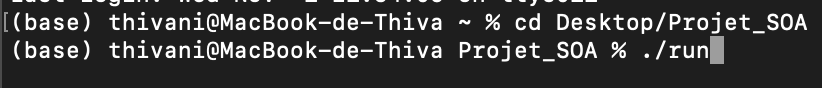
\includegraphics[width=\textwidth]{images/run.png} \\
		\\
		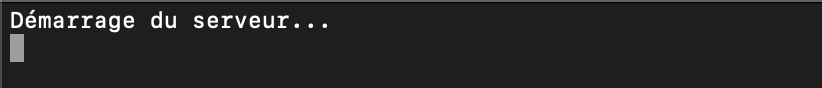
\includegraphics[width=\textwidth]{images/lancement.png}
		
		\item Interface Web accueil : \\
		\\
		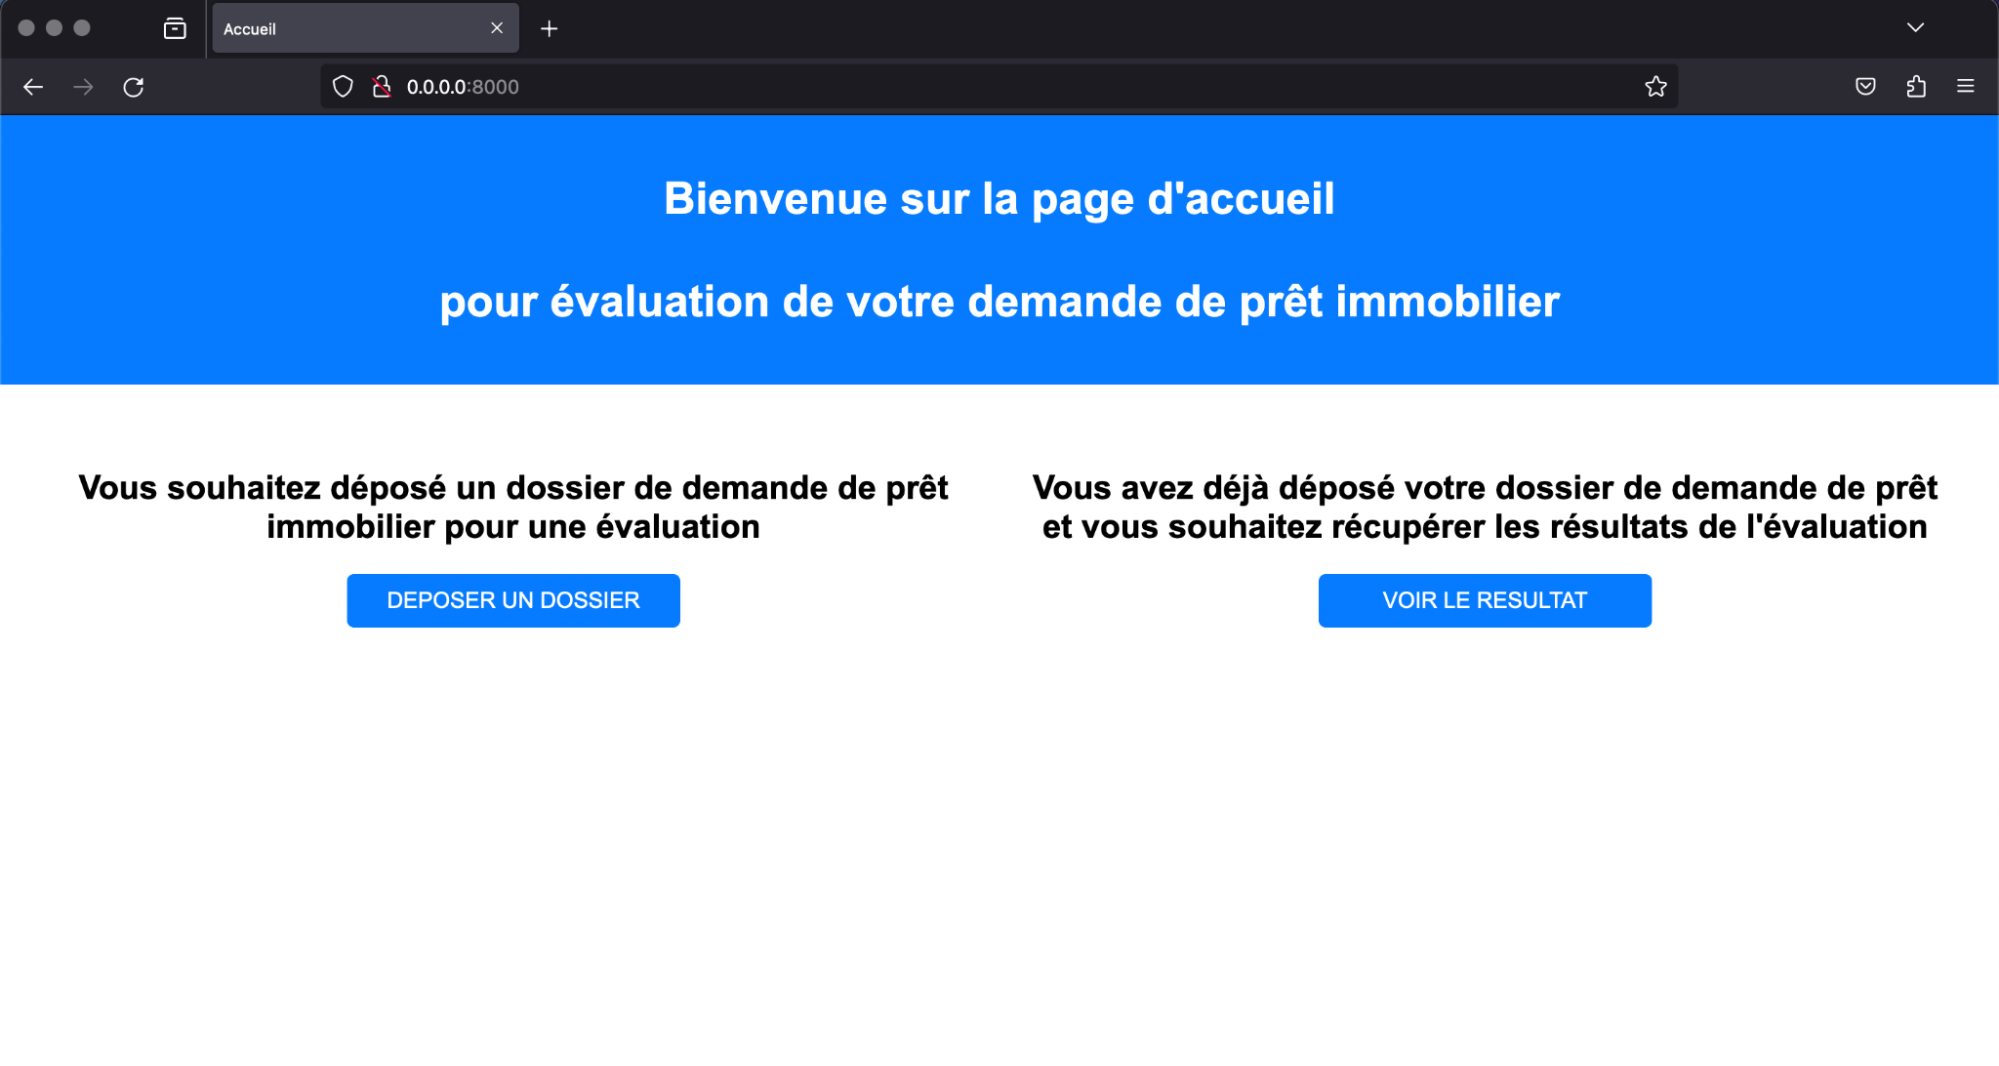
\includegraphics[width=\textwidth]{images/accueil.png}
	\end{itemize}
	
   \newpage
   \begin{itemize}

		
		\item Si l'utilisateur clique sur "Déposer un dossier", il est redirigé vers la page de formulaire : \\
		\\
		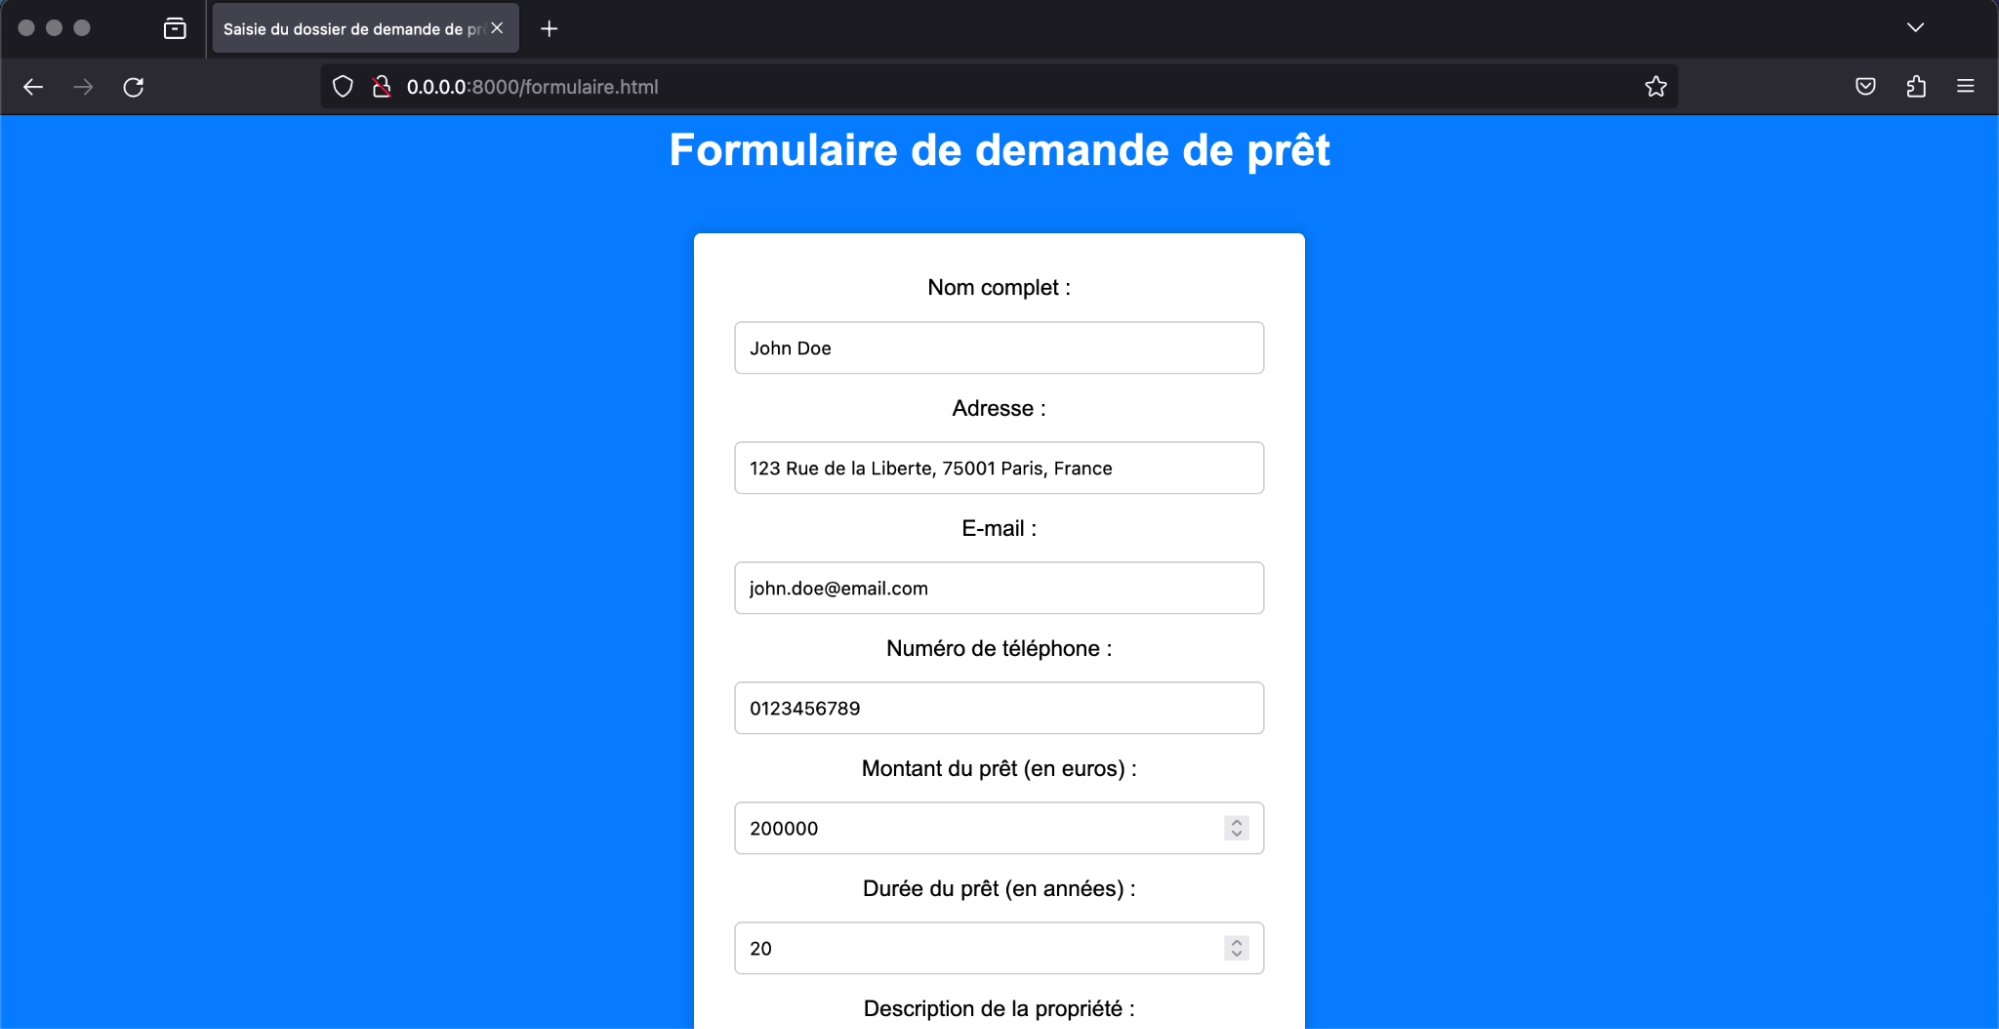
\includegraphics[width=\textwidth]{images/formulairea1.png} \\
		
\includegraphics[width=\textwidth]{images/formulairea2.png}
		
		\item Après avoir cliqué sur le bouton "Soumettre", la page confirmation s’ouvre : \\ 
		\\
		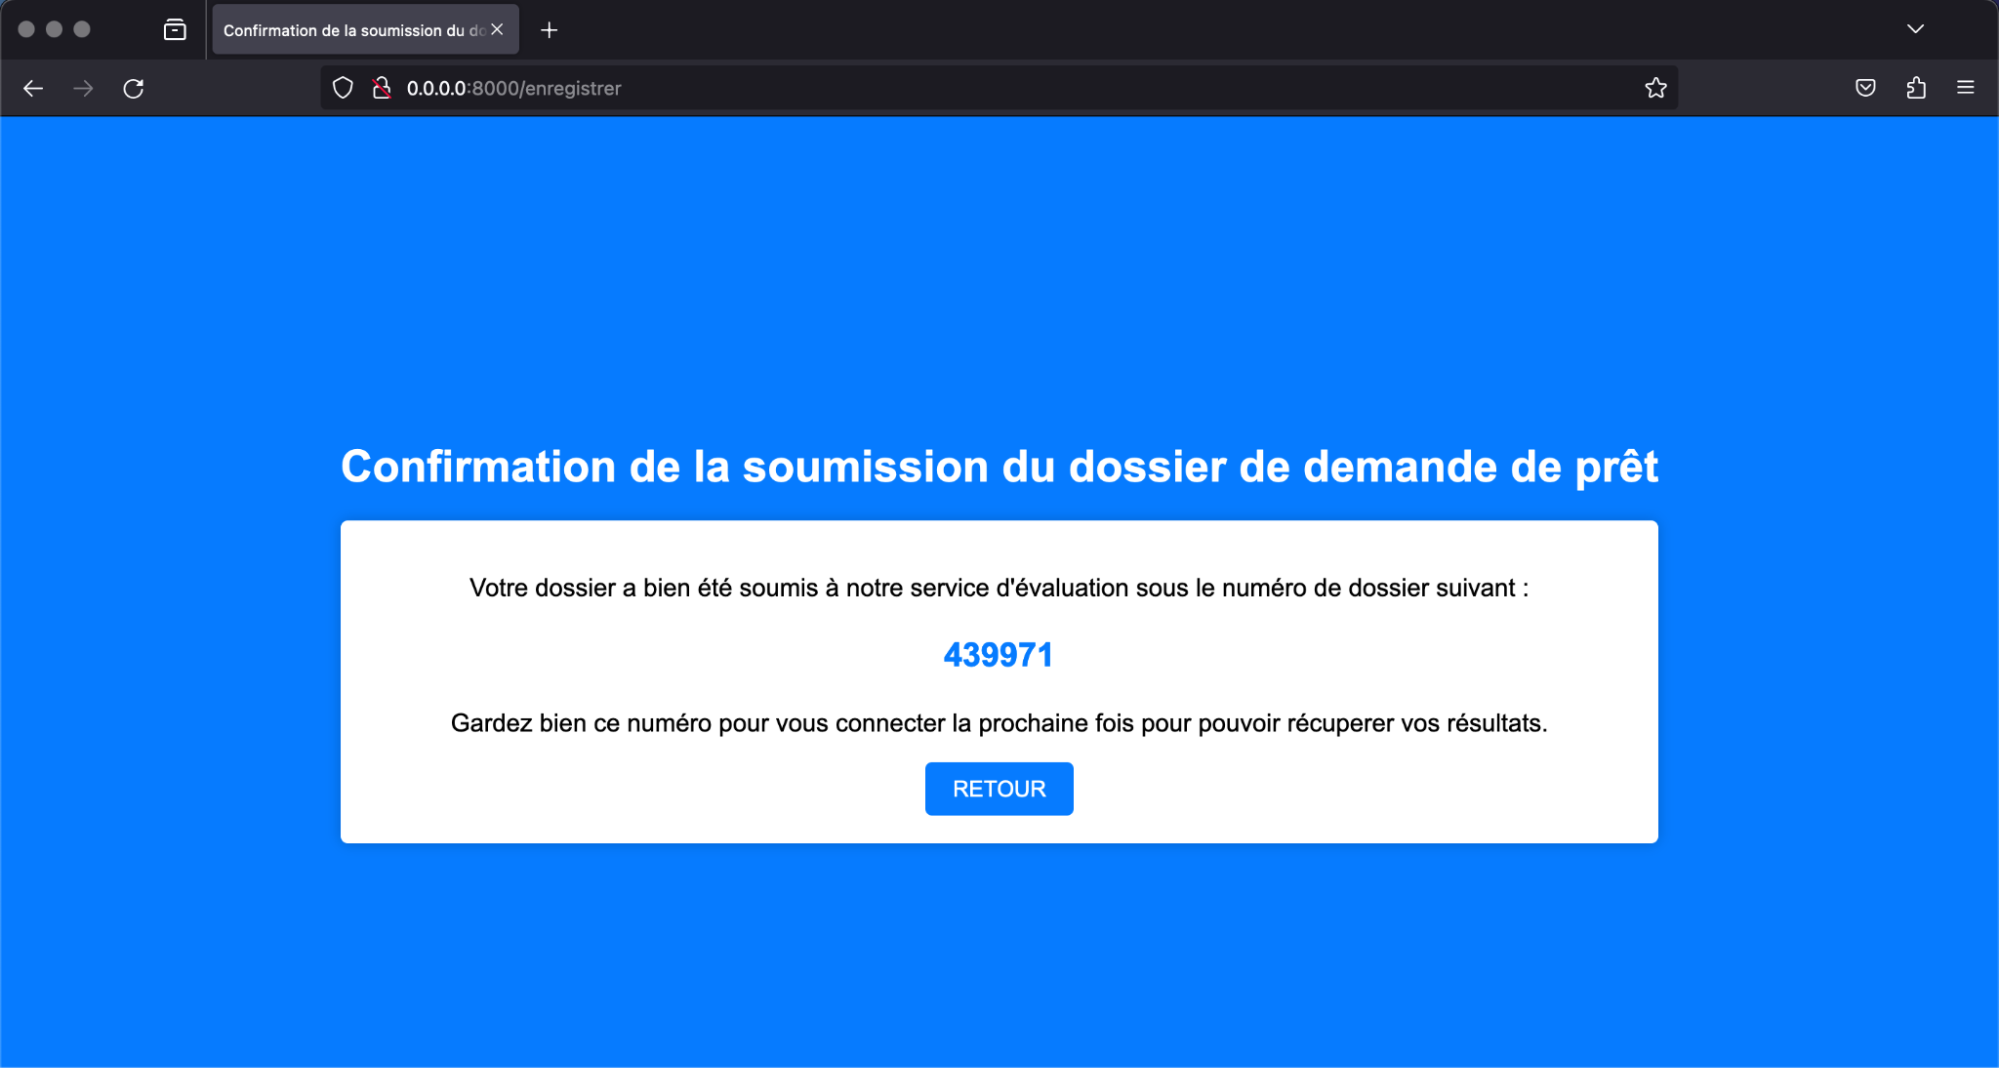
\includegraphics[width=\textwidth]{images/depota.png} \\
		\\
		Elle nous indique le numéro de dossier de la demande qui est à conserver pour pouvoir consulter les résultats par la suite
		
		\item Si l'utilisateur clique sur "Retour", il revient à la page d'accueil \\
		\\
		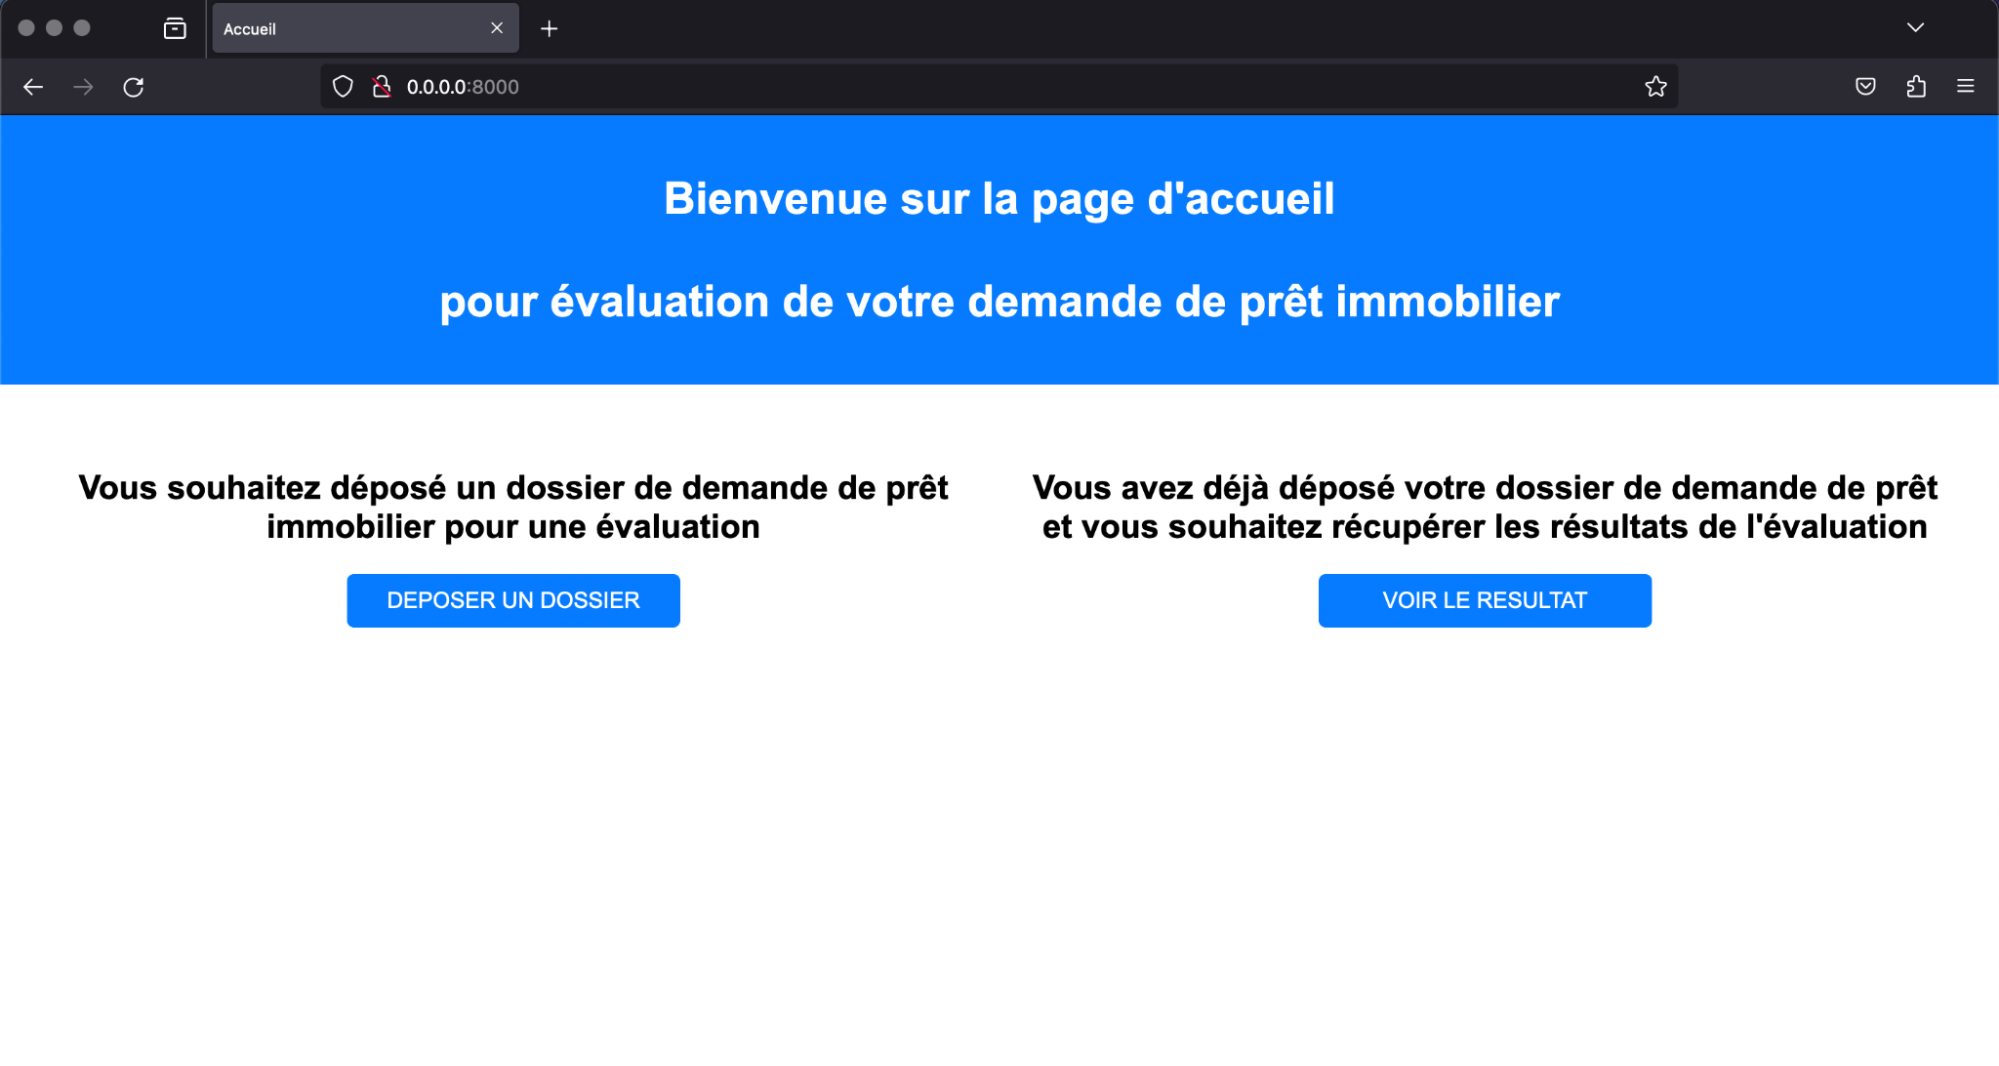
\includegraphics[width=\textwidth]{images/accueil.png}
		
		\item Si l'utilisateur clique sur le bouton "Voir le résultat", la page de connexion s'affiche \\
		\\
	   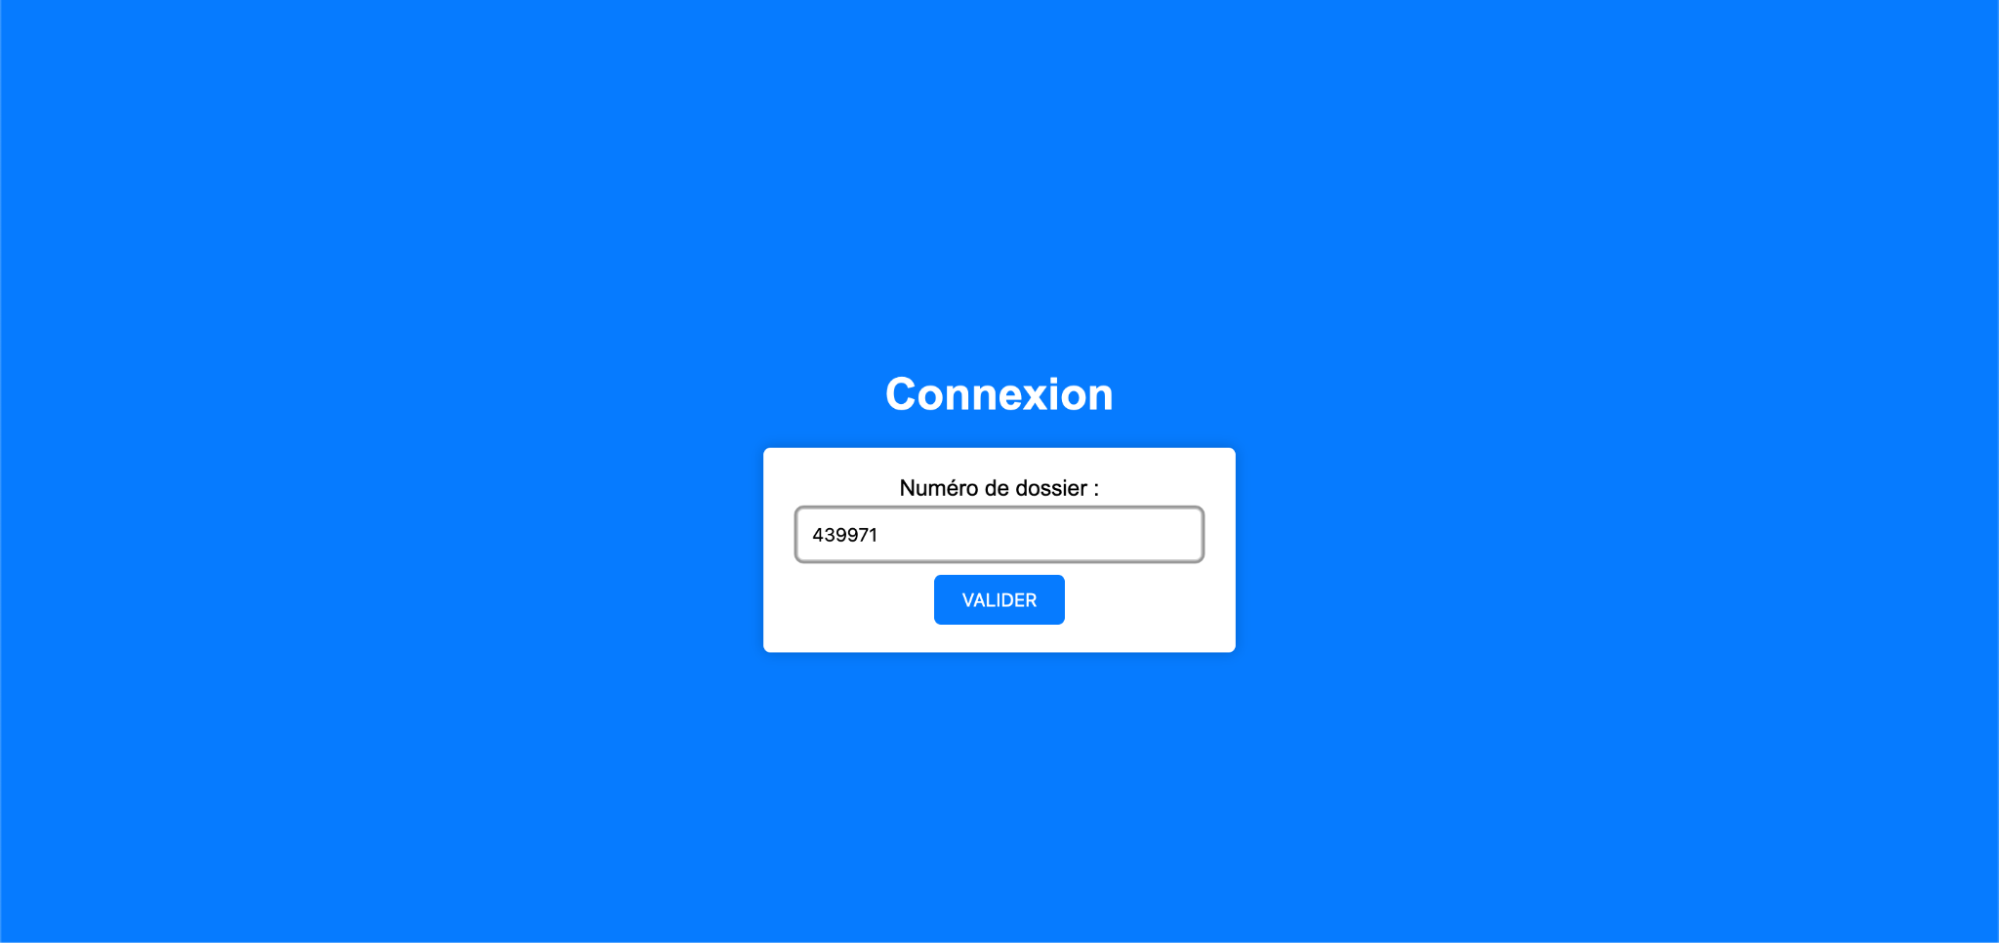
\includegraphics[width=\textwidth]{images/connexiona.png}  \\
	   \\
	   L'utilisateur saisit donc son numéro de dossier 
		
	   \item L'utilisateur accède à la page de confirmation de la demande de prêt : \\
	   \\
	   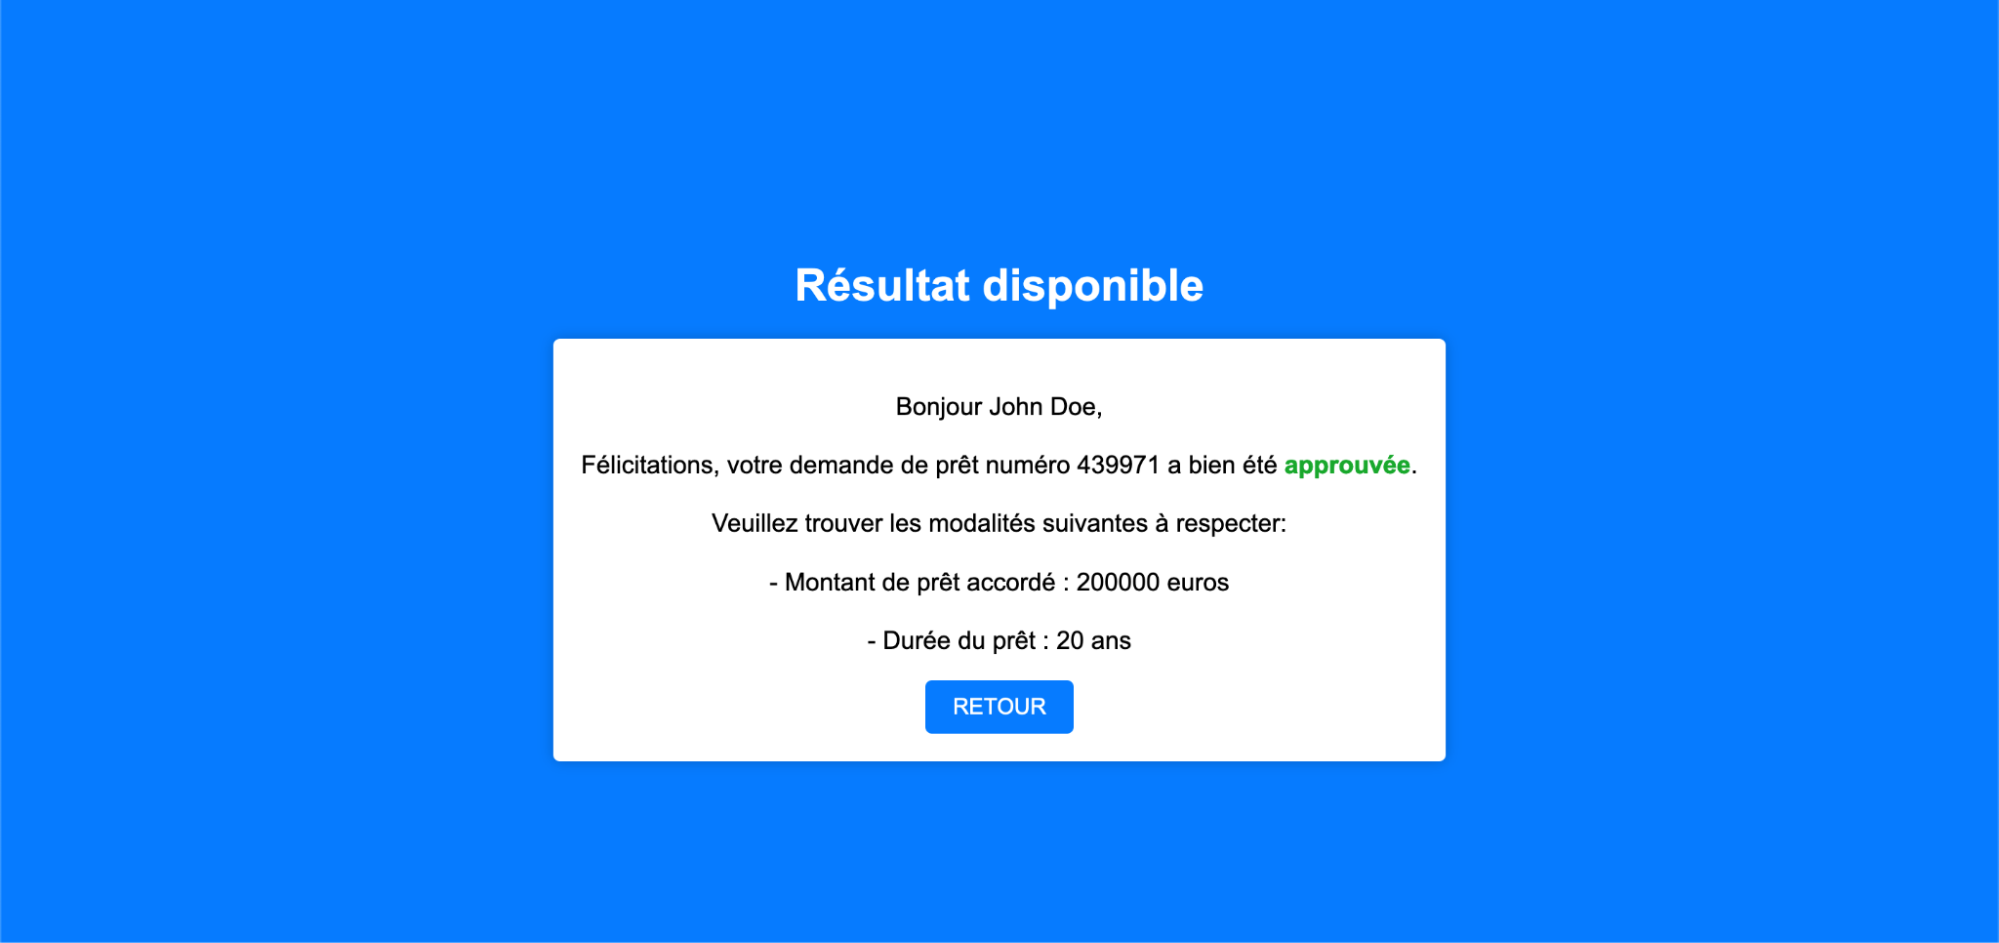
\includegraphics[width=\textwidth]{images/confirmationa.png} \\
	   \\
	   Sur celle-ci y figure les modalités à respecter
	   
	   \item Voici la même demande avec un dossier refusé : \\
	   \\
	   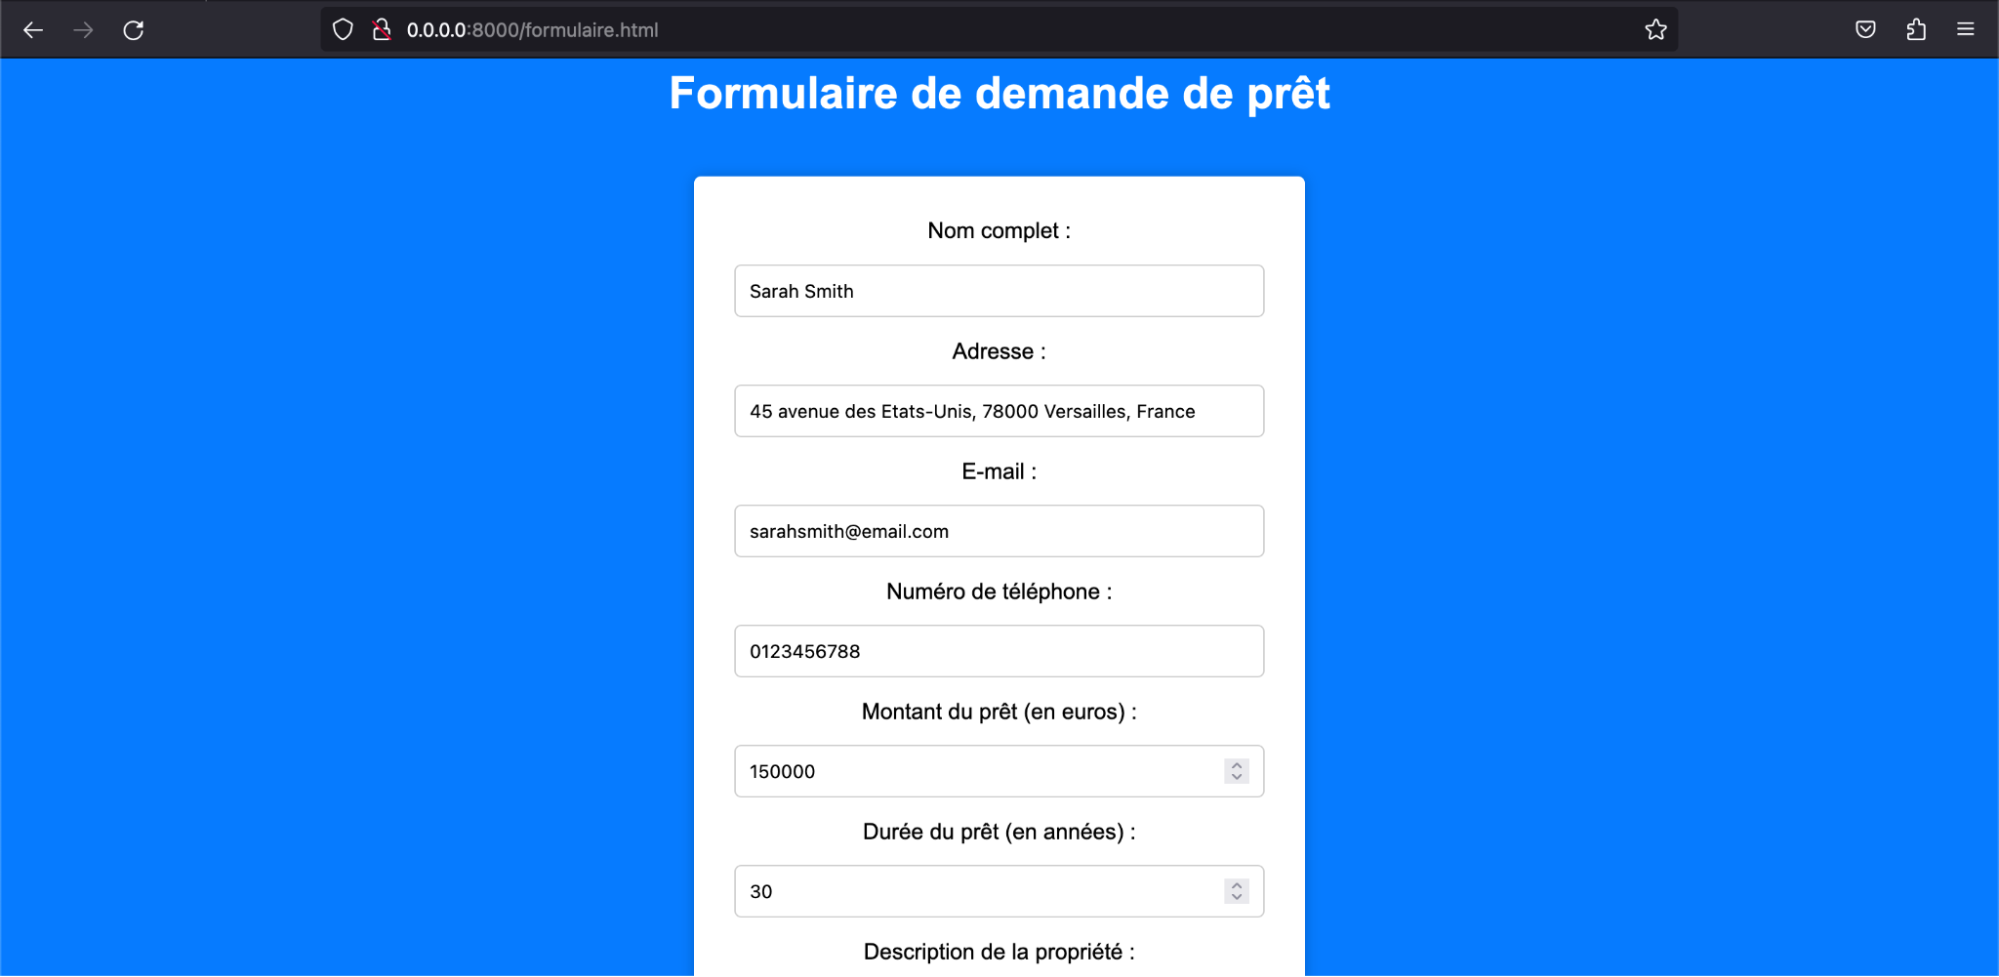
\includegraphics[width=\textwidth]{images/formulairera.png} \\
	   
\includegraphics[width=\textwidth]{images/formulairerb.png} \\
	   \\
	   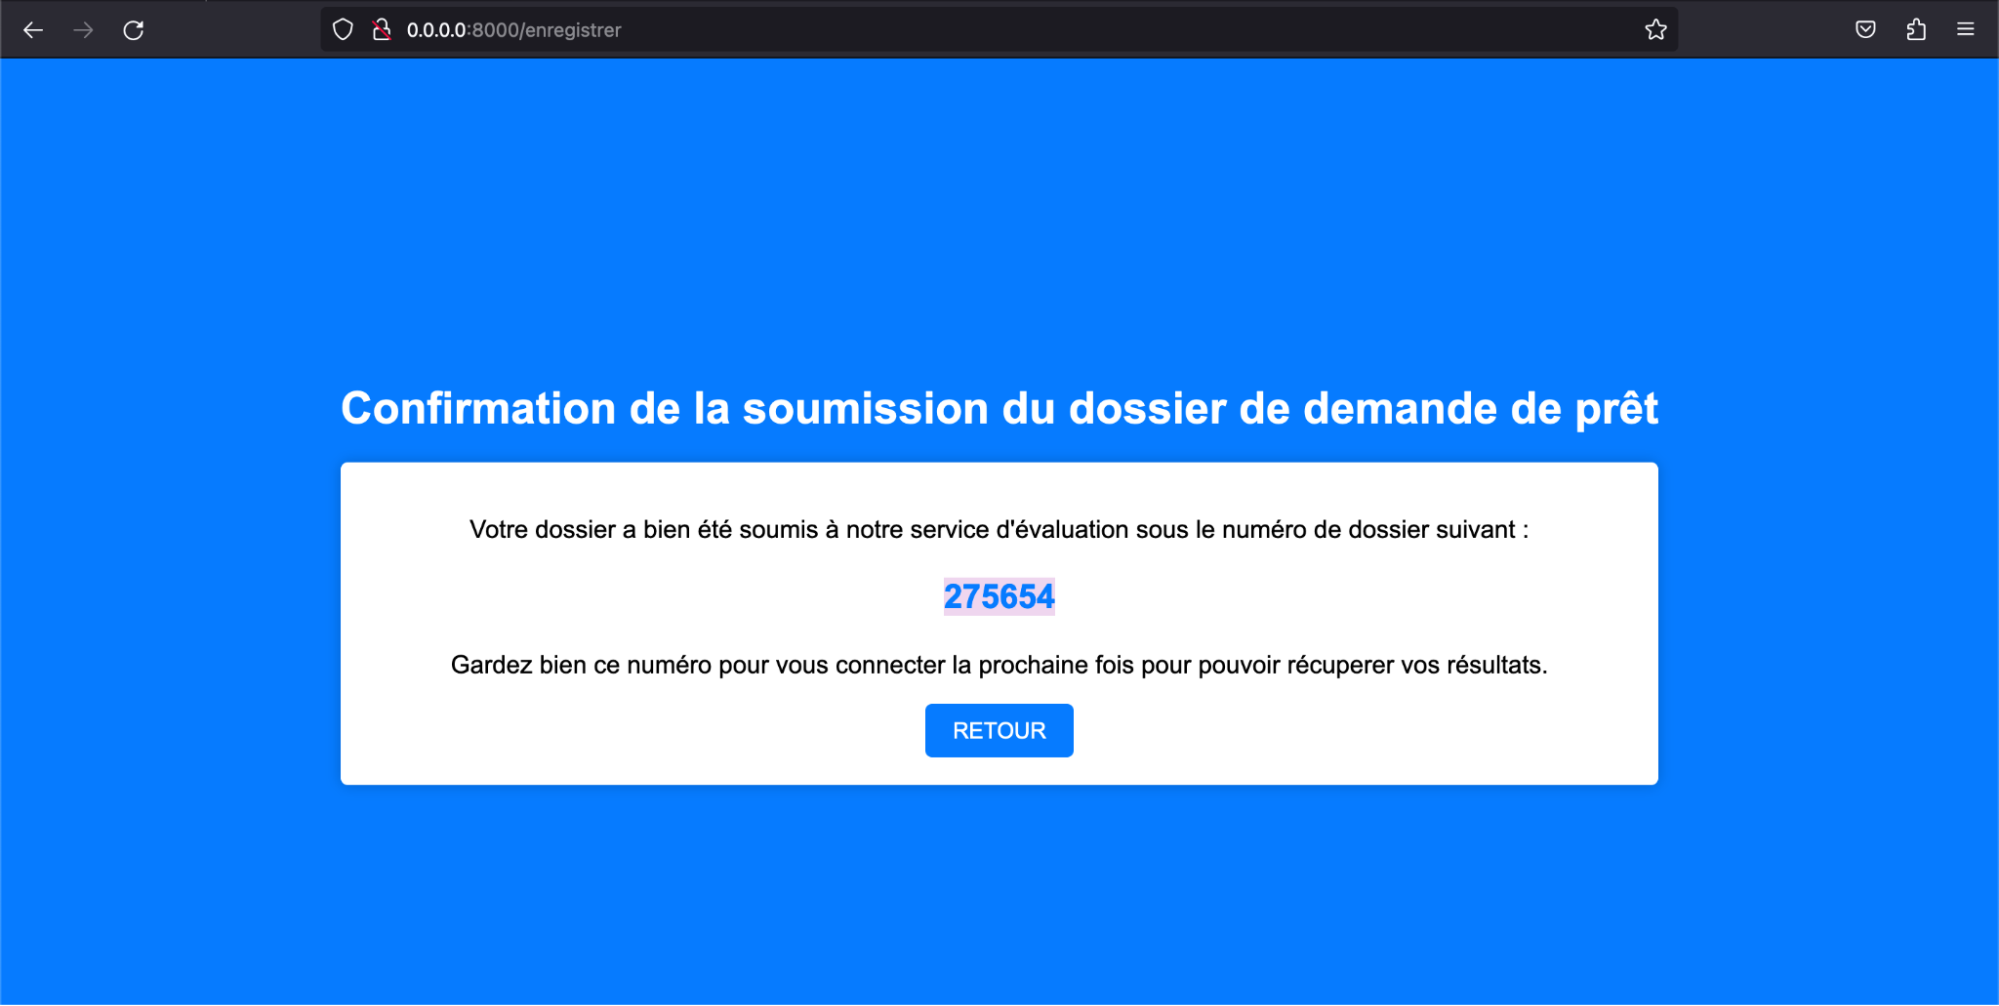
\includegraphics[width=\textwidth]{images/depotr.png} \\
	   \\
	   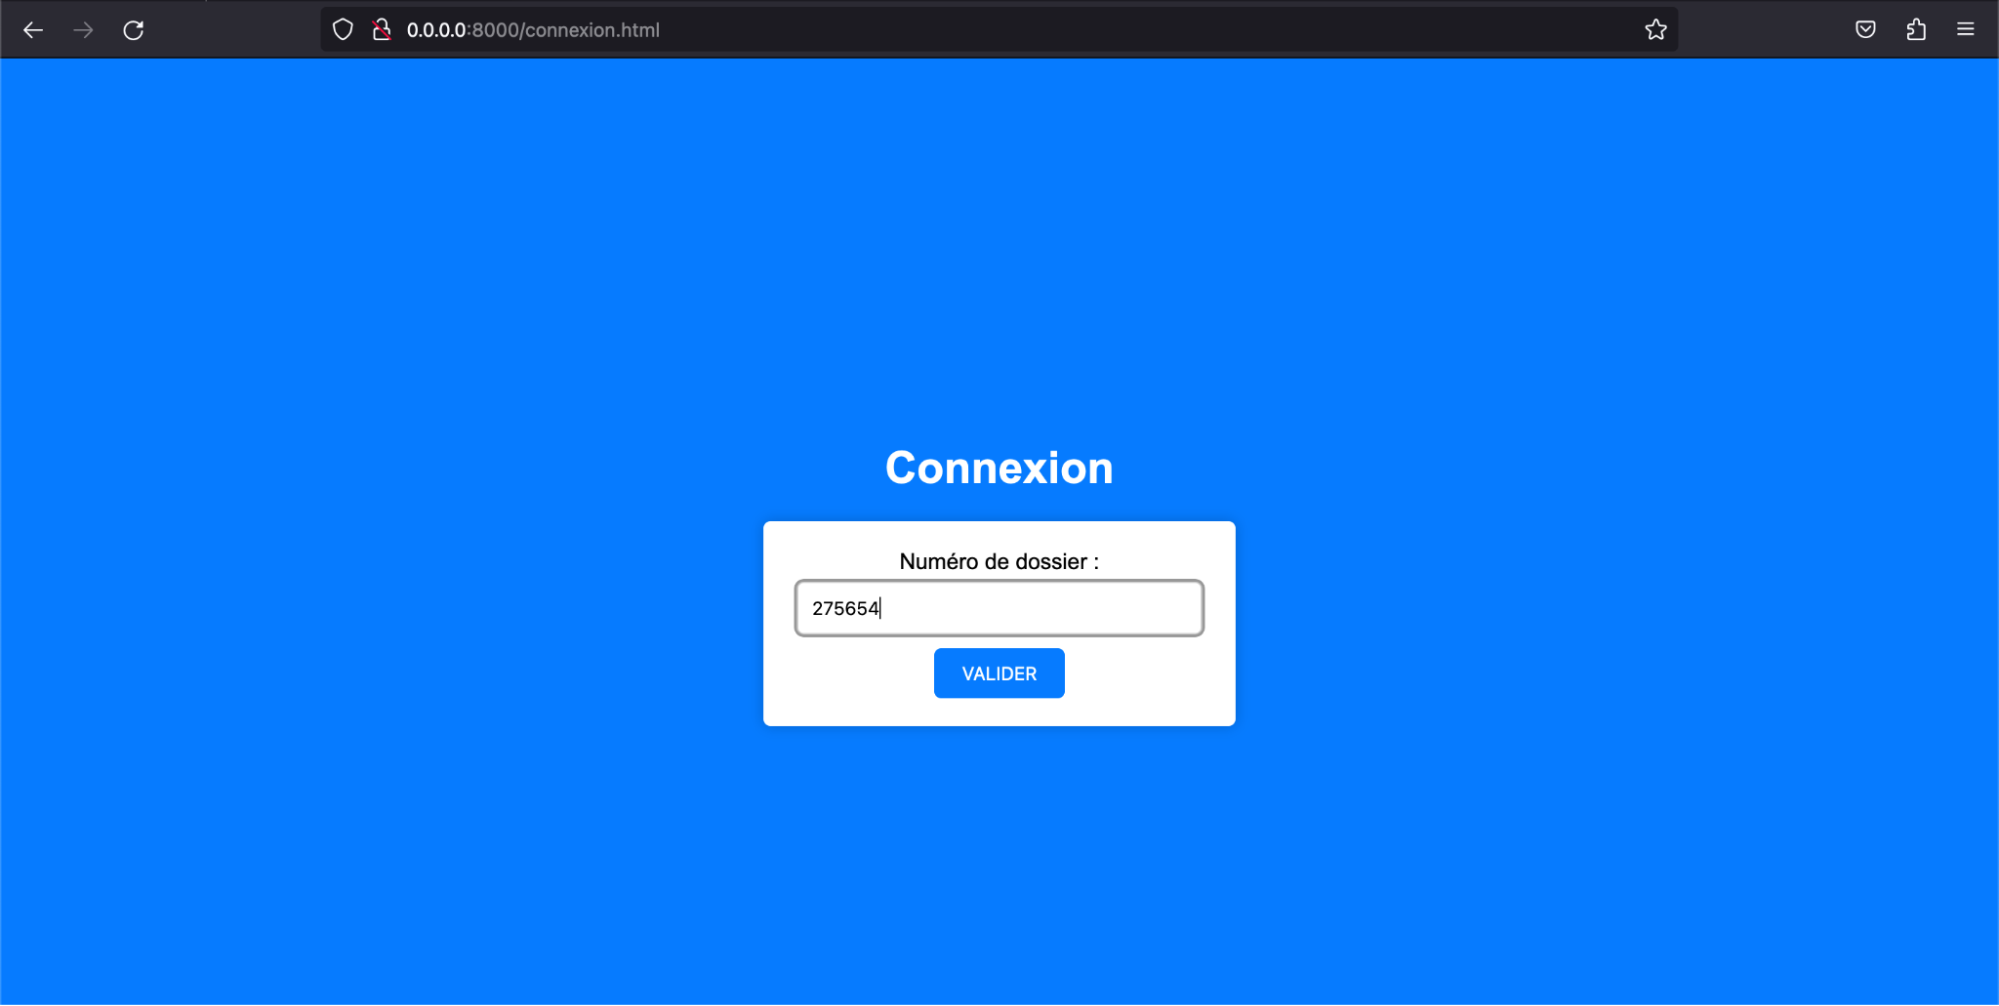
\includegraphics[width=\textwidth]{images/connexionr.png} \\
	   \\
	   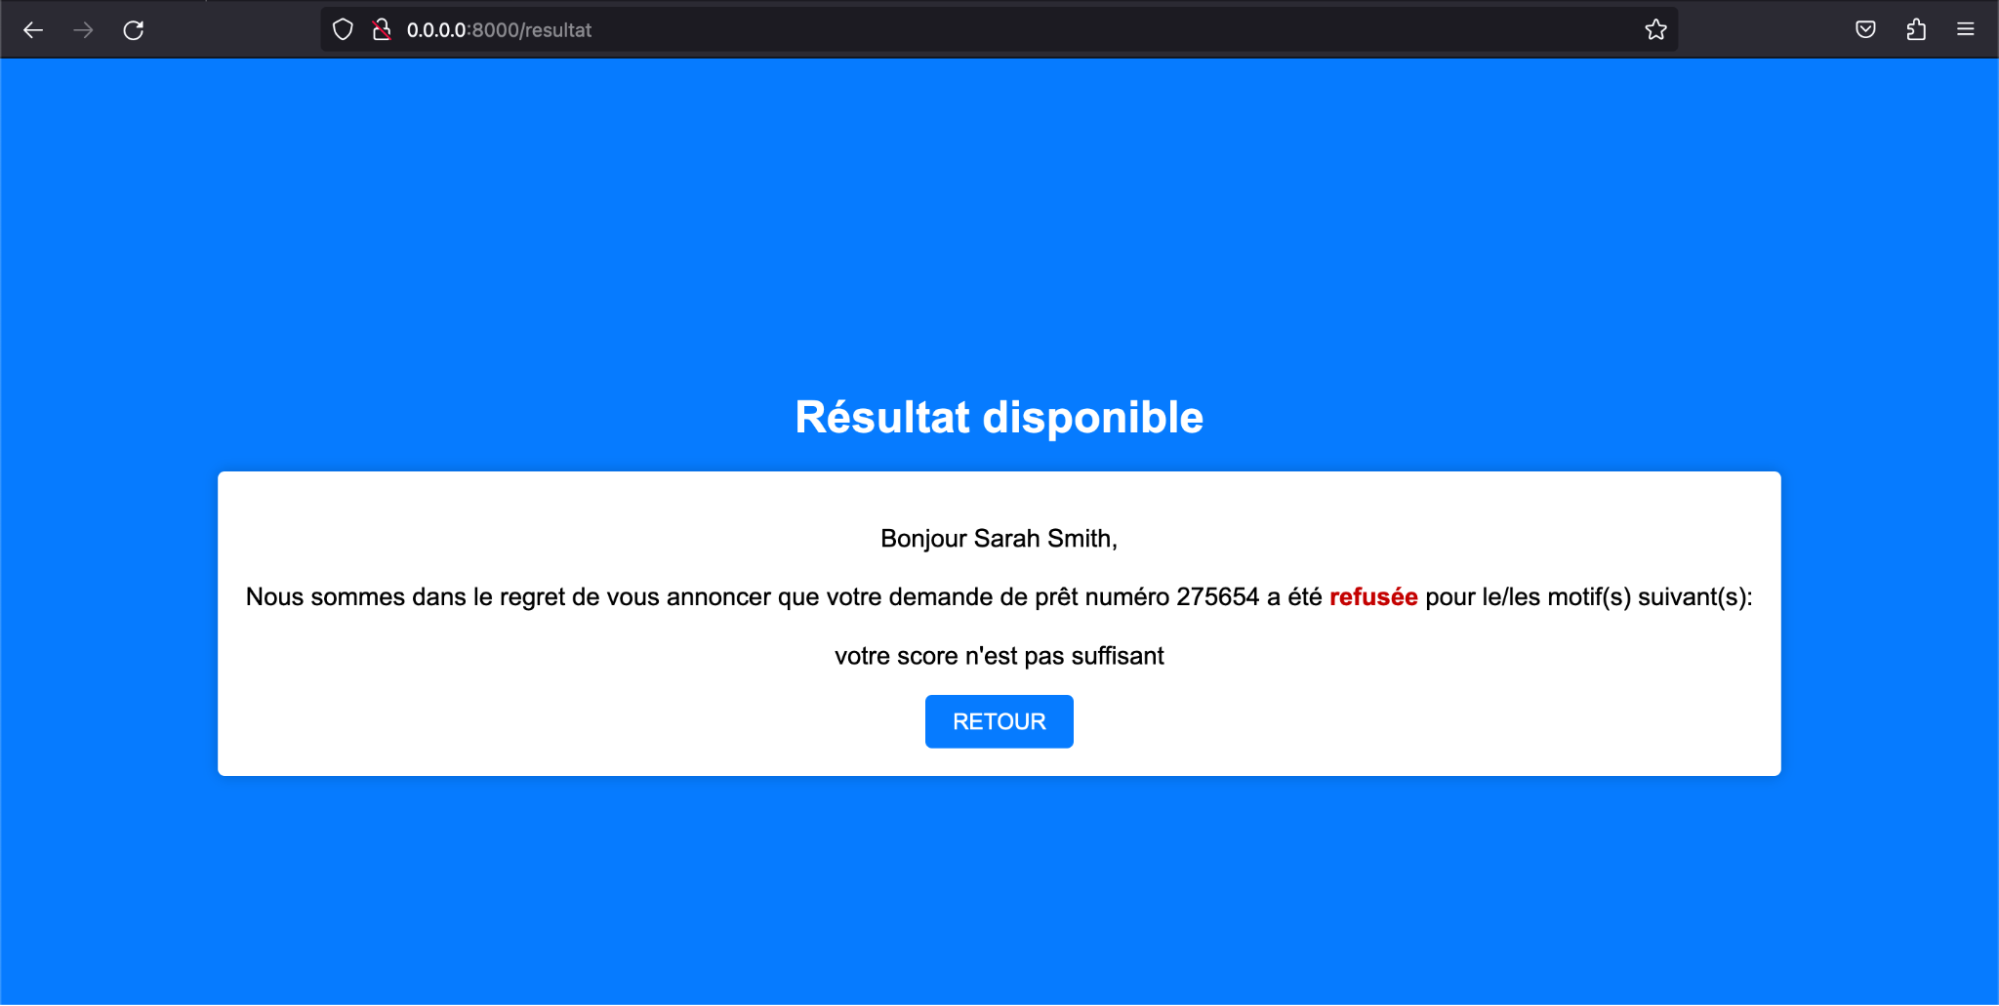
\includegraphics[width=\textwidth]{images/confirmationr.png}
   
	\end{itemize}
	\subsection{Cas à tester}
	\newpage
	\section{Liens des dépôts du projet}
	 \begin{itemize}
	 	\item \textcolor{blue}{\href{https://github.com/uvsq21704755/ProjetSOAP.git}{SOAP}} : \texttt{https://github.com/uvsq21704755/ProjetSOAP.git}
	 	\item \textcolor{blue}{\href{https://github.com/uvsq21704755/ProjetREST.git}{REST}} : \texttt{https://github.com/uvsq21704755/Projet\_REST.git}
	 \end{itemize}
	

	
\end{document}